% Options for packages loaded elsewhere
\PassOptionsToPackage{unicode}{hyperref}
\PassOptionsToPackage{hyphens}{url}
%
\documentclass[
  english,
  man]{apa6}
\usepackage{amsmath,amssymb}
\usepackage{lmodern}
\usepackage{ifxetex,ifluatex}
\ifnum 0\ifxetex 1\fi\ifluatex 1\fi=0 % if pdftex
  \usepackage[T1]{fontenc}
  \usepackage[utf8]{inputenc}
  \usepackage{textcomp} % provide euro and other symbols
\else % if luatex or xetex
  \usepackage{unicode-math}
  \defaultfontfeatures{Scale=MatchLowercase}
  \defaultfontfeatures[\rmfamily]{Ligatures=TeX,Scale=1}
  \setmainfont[]{Times New Roman}
\fi
% Use upquote if available, for straight quotes in verbatim environments
\IfFileExists{upquote.sty}{\usepackage{upquote}}{}
\IfFileExists{microtype.sty}{% use microtype if available
  \usepackage[]{microtype}
  \UseMicrotypeSet[protrusion]{basicmath} % disable protrusion for tt fonts
}{}
\makeatletter
\@ifundefined{KOMAClassName}{% if non-KOMA class
  \IfFileExists{parskip.sty}{%
    \usepackage{parskip}
  }{% else
    \setlength{\parindent}{0pt}
    \setlength{\parskip}{6pt plus 2pt minus 1pt}}
}{% if KOMA class
  \KOMAoptions{parskip=half}}
\makeatother
\usepackage{xcolor}
\IfFileExists{xurl.sty}{\usepackage{xurl}}{} % add URL line breaks if available
\IfFileExists{bookmark.sty}{\usepackage{bookmark}}{\usepackage{hyperref}}
\hypersetup{
  pdftitle={DoPL},
  pdfauthor={Ithurburn, Andrew1, Pedersen, Julie1, \& Moore, Adam1},
  pdflang={en-EN},
  pdfkeywords={keywords},
  hidelinks,
  pdfcreator={LaTeX via pandoc}}
\urlstyle{same} % disable monospaced font for URLs
\usepackage{graphicx}
\makeatletter
\def\maxwidth{\ifdim\Gin@nat@width>\linewidth\linewidth\else\Gin@nat@width\fi}
\def\maxheight{\ifdim\Gin@nat@height>\textheight\textheight\else\Gin@nat@height\fi}
\makeatother
% Scale images if necessary, so that they will not overflow the page
% margins by default, and it is still possible to overwrite the defaults
% using explicit options in \includegraphics[width, height, ...]{}
\setkeys{Gin}{width=\maxwidth,height=\maxheight,keepaspectratio}
% Set default figure placement to htbp
\makeatletter
\def\fps@figure{htbp}
\makeatother
\setlength{\emergencystretch}{3em} % prevent overfull lines
\providecommand{\tightlist}{%
  \setlength{\itemsep}{0pt}\setlength{\parskip}{0pt}}
\setcounter{secnumdepth}{-\maxdimen} % remove section numbering
% Make \paragraph and \subparagraph free-standing
\ifx\paragraph\undefined\else
  \let\oldparagraph\paragraph
  \renewcommand{\paragraph}[1]{\oldparagraph{#1}\mbox{}}
\fi
\ifx\subparagraph\undefined\else
  \let\oldsubparagraph\subparagraph
  \renewcommand{\subparagraph}[1]{\oldsubparagraph{#1}\mbox{}}
\fi
% Manuscript styling
\usepackage{upgreek}
\captionsetup{font=singlespacing,justification=justified}

% Table formatting
\usepackage{longtable}
\usepackage{lscape}
% \usepackage[counterclockwise]{rotating}   % Landscape page setup for large tables
\usepackage{multirow}		% Table styling
\usepackage{tabularx}		% Control Column width
\usepackage[flushleft]{threeparttable}	% Allows for three part tables with a specified notes section
\usepackage{threeparttablex}            % Lets threeparttable work with longtable

% Create new environments so endfloat can handle them
% \newenvironment{ltable}
%   {\begin{landscape}\begin{center}\begin{threeparttable}}
%   {\end{threeparttable}\end{center}\end{landscape}}
\newenvironment{lltable}{\begin{landscape}\begin{center}\begin{ThreePartTable}}{\end{ThreePartTable}\end{center}\end{landscape}}

% Enables adjusting longtable caption width to table width
% Solution found at http://golatex.de/longtable-mit-caption-so-breit-wie-die-tabelle-t15767.html
\makeatletter
\newcommand\LastLTentrywidth{1em}
\newlength\longtablewidth
\setlength{\longtablewidth}{1in}
\newcommand{\getlongtablewidth}{\begingroup \ifcsname LT@\roman{LT@tables}\endcsname \global\longtablewidth=0pt \renewcommand{\LT@entry}[2]{\global\advance\longtablewidth by ##2\relax\gdef\LastLTentrywidth{##2}}\@nameuse{LT@\roman{LT@tables}} \fi \endgroup}

% \setlength{\parindent}{0.5in}
% \setlength{\parskip}{0pt plus 0pt minus 0pt}

% \usepackage{etoolbox}
\makeatletter
\patchcmd{\HyOrg@maketitle}
  {\section{\normalfont\normalsize\abstractname}}
  {\section*{\normalfont\normalsize\abstractname}}
  {}{\typeout{Failed to patch abstract.}}
\patchcmd{\HyOrg@maketitle}
  {\section{\protect\normalfont{\@title}}}
  {\section*{\protect\normalfont{\@title}}}
  {}{\typeout{Failed to patch title.}}
\makeatother
\shorttitle{Title}
\keywords{keywords\newline\indent Word count: 591}
\DeclareDelayedFloatFlavor{ThreePartTable}{table}
\DeclareDelayedFloatFlavor{lltable}{table}
\DeclareDelayedFloatFlavor*{longtable}{table}
\makeatletter
\renewcommand{\efloat@iwrite}[1]{\immediate\expandafter\protected@write\csname efloat@post#1\endcsname{}}
\makeatother
\usepackage{lineno}

\linenumbers
\usepackage{csquotes}
\raggedbottom
\ifxetex
  % Load polyglossia as late as possible: uses bidi with RTL langages (e.g. Hebrew, Arabic)
  \usepackage{polyglossia}
  \setmainlanguage[]{english}
\else
  \usepackage[main=english]{babel}
% get rid of language-specific shorthands (see #6817):
\let\LanguageShortHands\languageshorthands
\def\languageshorthands#1{}
\fi
\ifluatex
  \usepackage{selnolig}  % disable illegal ligatures
\fi
\newlength{\cslhangindent}
\setlength{\cslhangindent}{1.5em}
\newlength{\csllabelwidth}
\setlength{\csllabelwidth}{3em}
\newenvironment{CSLReferences}[2] % #1 hanging-ident, #2 entry spacing
 {% don't indent paragraphs
  \setlength{\parindent}{0pt}
  % turn on hanging indent if param 1 is 1
  \ifodd #1 \everypar{\setlength{\hangindent}{\cslhangindent}}\ignorespaces\fi
  % set entry spacing
  \ifnum #2 > 0
  \setlength{\parskip}{#2\baselineskip}
  \fi
 }%
 {}
\usepackage{calc}
\newcommand{\CSLBlock}[1]{#1\hfill\break}
\newcommand{\CSLLeftMargin}[1]{\parbox[t]{\csllabelwidth}{#1}}
\newcommand{\CSLRightInline}[1]{\parbox[t]{\linewidth - \csllabelwidth}{#1}\break}
\newcommand{\CSLIndent}[1]{\hspace{\cslhangindent}#1}

\title{DoPL}
\author{Ithurburn, Andrew\textsuperscript{1}, Pedersen, Julie\textsuperscript{1}, \& Moore, Adam\textsuperscript{1}}
\date{}


\authornote{

The authors made the following contributions. Ithurburn, Andrew: Conceptualization, Writing - Original Draft Preparation, Writing - Review \& Editing; Moore, Adam: Writing - Review \& Editing.

Correspondence concerning this article should be addressed to Ithurburn, Andrew, 7 George Square, Edinburgh, EH8 9JZ. E-mail: \href{mailto:a.ithurburn@sms.ed.ac.uk}{\nolinkurl{a.ithurburn@sms.ed.ac.uk}}

}

\affiliation{\vspace{0.5cm}\textsuperscript{1} The University of Edinburgh}

\begin{document}
\maketitle

\hypertarget{introduction}{%
\section{Introduction}\label{introduction}}

\hypertarget{dominance-leadership-and-prestige-orientation}{%
\subsection{Dominance, Leadership, and Prestige orientation}\label{dominance-leadership-and-prestige-orientation}}

\hypertarget{risk}{%
\subsection{Risk}\label{risk}}

\hypertarget{domain-specific-risk-taking}{%
\subsection{Domain Specific Risk-taking}\label{domain-specific-risk-taking}}

\hypertarget{the-present-study}{%
\subsection{The present study}\label{the-present-study}}

\hypertarget{methods}{%
\section{Methods}\label{methods}}

Participants were a convenience sample of 111 individuals from Prolific Academic's crowdsourcing platform (www.prolific.io). Prolific Academic is an online crowdsourcing service that provides participants access to studies hosted on third party websites. Participants were required to be 18 years of age or older and be able to read and understand English. Participants received £4.00, which is above the current minimum wage pro-rata in the United Kingdom, as compensation for completing the survey. The Psychology Research Ethics Committee at the University of Edinburgh approved all study procedures {[}ref: \#\#\#\#{]}. The present study was pre-registered along with a copy of anonymized data and copy of R code is available at (\url{https://osf.io/s4j7y}).

\hypertarget{materials}{%
\subsection{Materials}\label{materials}}

\emph{Demographic Questionnaire}. In a demographic questionnaire administered prior to the main survey, participants were invited to respond to questions about their self-identified demographic characteristics such as gender, ethnicity, and ethnic origin.

\emph{Dominance, Prestige, and Leadership Orientation}. The 18-item Dominance, Prestige, and Leadership scale {[}DoPL; Suessenbach, Loughnan, Schönbrodt, and Moore (2019){]}, is used to measure dominance, prestige, and leadership orientation. Each question corresponds to one of the three domains. Each domain is scored across six unique items related to those domains (e.g., ``I relish opportunities in which I can lead others'' for leadership) rated on a scale from 0 (Strongly disagree) to 5 (Strongly agree). Internal consistency reliability for the current sample is \(\alpha\) = 0.86.

\emph{Domain Specific Risk-taking Scale} (DOSPERT; Weber, Blais, and Betz (2002)) is a scale assessing individuals' likelihood of engaging in risky behaviors within 5 domain specific risky situations: financial, social, recreational, health and safety, and ethical situations. Each risky situation is then rated on a five-point Likert scale (1 being very unlikely and 5 being very likely). Two additional five-point Likert scales assess risk perception and expected benefits (1 being not at all risky and 5 being extremely risky; 1 being no benefits at all and 5 being great benefits) respectively. Example risky situations are ``Admitting that your tastes are different from those of a friend'' and ``Drinking heavily at a social function.'' Internal consistency reliability for the current samples for the 3 sub-domains are \(\alpha\) = 0.85, \(\alpha\) = 0.90, \(\alpha\) = 0.92 respectively.

\hypertarget{procedure}{%
\subsection{Procedure}\label{procedure}}

Participants were recruited via a study landing page on Prolific's website or via a direct e-mail to eligible participants (Prolific FAQ, 2018). The study landing page included a brief description of the study including any risks and benefits along with expected compensation for successful completion. Participants accepted participation in the experiment and were directed to the main survey (Qualtrics, Inc; Provo, UT) where they were shown a brief message on study consent.

Once participants consented to participate in the experiment they answered a series of demographic questions. Once completed, participants completed the Dominance, Prestige, and Leadership Scale and the Domain Specific Risk-taking scale. The two scales were counterbalanced to account for order effects. After completion of the main survey, participants were shown a debriefing statement that briefly mentions the purpose of the experiment along with the contact information of the main researcher (AI). Participants were compensated £4.00 via Prolific Academic.

\hypertarget{data-analysis}{%
\subsection{Data analysis}\label{data-analysis}}

Demographic characteristics were analyzed using a multiple regression for continuous variables (age) and Chi-square tests for categorical variables (gender, race, ethnicity, ethnic origin, and education). Means and standard deviations were calculated for the relevant scales (i.e., DoPL and DOSPERT). All analyses were done using (R Core Team, 2021) along with (Stan Development Team, 2020) package.

\hypertarget{results}{%
\section{Results}\label{results}}

One hundred and eleven individuals completed the main survey. Of these individuals, 111 completed all sections without incomplete data and were therefore retained in most data analyses. In later analyses to account for outliers two participants had to be excluded from the dataset. Table 1 shows the demographic information for the participants. Average completion time for participants was 16M 49S(\emph{SD} = 43.79).

\hypertarget{preregistered-analyses}{%
\subsection{Preregistered Analyses}\label{preregistered-analyses}}

We first DoPL orientation on general risk preference (Figure 1). General risk preference was

All participants completed the dominance, leadership, and prestige scale (Suessenbach, Loughnan, Schönbrodt, and Moore (2019)). Empirically, men have generally been more dominance oriented in their behavior (citation). Following the literature, men tended to be more dominance oriented than women ()

\hypertarget{domain-specific-risk-taking-1}{%
\subsection{Domain Specific Risk-Taking}\label{domain-specific-risk-taking-1}}

\hypertarget{interactions}{%
\subsection{Interactions}\label{interactions}}

\hypertarget{discussion}{%
\section{Discussion}\label{discussion}}

\newpage

\hypertarget{references}{%
\section{References}\label{references}}

\begingroup
\setlength{\parindent}{-0.5in}
\setlength{\leftskip}{0.5in}

\hypertarget{refs}{}
\begin{CSLReferences}{1}{0}
\leavevmode\hypertarget{ref-R-base}{}%
R Core Team. (2021). \emph{R: A language and environment for statistical computing}. Vienna, Austria: R Foundation for Statistical Computing. Retrieved from \url{https://www.R-project.org/}

\leavevmode\hypertarget{ref-rStan}{}%
Stan Development Team. (2020). {RStan}: The {R} interface to {Stan}. Retrieved from \url{http://mc-stan.org/}

\leavevmode\hypertarget{ref-suessenbach_dominance_2019}{}%
Suessenbach, F., Loughnan, S., Schönbrodt, F. D., \& Moore, A. B. (2019). The dominance, prestige, and leadership account of social power motives. \emph{European Journal of Personality}, \emph{33}(1), 7--33. \url{https://doi.org/10.1002/per.2184}

\leavevmode\hypertarget{ref-weber_domain-specific_2002}{}%
Weber, E. U., Blais, A.-R., \& Betz, N. E. (2002). A domain-specific risk-attitude scale: Measuring risk perceptions and risk behaviors. \emph{Journal of Behavioral Decision Making}, \emph{15}(4), 263--290. \url{https://doi.org/10.1002/bdm.414}

\end{CSLReferences}

\endgroup

\newpage

\hypertarget{figures-and-tables}{%
\section{Figures and Tables}\label{figures-and-tables}}

\begin{table}[tbp]

\begin{center}
\begin{threeparttable}

\caption{\label{tab:unnamed-chunk-1}}

\begin{tabular}{ll}
\toprule
Variables & \\
\midrule
NA & n = 111\\
Age & \\
\ \ \ Mean (SD) & 26.8 (9.2)\\
\ \ \ Median [Min, Max] & 24 [18, 61]\\
Gender & \\
\ \ \ Female & 54 (48.6\%)\\
\ \ \ Gender Non-Binary & 2 (1.8\%)\\
\ \ \ Male & 55 (49.5\%)\\
Ethnicity & \\
\ \ \ Scottish & 2 (1.8\%)\\
\ \ \ English & 10 (9.0\%)\\
\ \ \ European & 77 (69.4\%)\\
\ \ \ Latin American & 2 (1.8\%)\\
\ \ \ Asian & 6 (5.4\%)\\
\ \ \ Arab & 0 (0.0\%)\\
\ \ \ African & 8 (7.2\%)\\
\ \ \ Other & 6 (5.4\%)\\
\ \ \ Prefer not to respond & 0 (0.0\%)\\
Education & \\
\ \ \ Primary School & 4 (3.6\%)\\
\ \ \ GCSes or Equivalent & 8 (7.2\%)\\
\ \ \ A-Levels or Equivalent & 32 (28.8\%)\\
\ \ \ University Undergraduate Program & 44 (39.6\%)\\
\ \ \ University Postgraduate Program & 21 (18.9\%)\\
\ \ \ Doctoral Degree & 1 (0.9\%)\\
\bottomrule
\end{tabular}

\end{threeparttable}
\end{center}

\end{table}

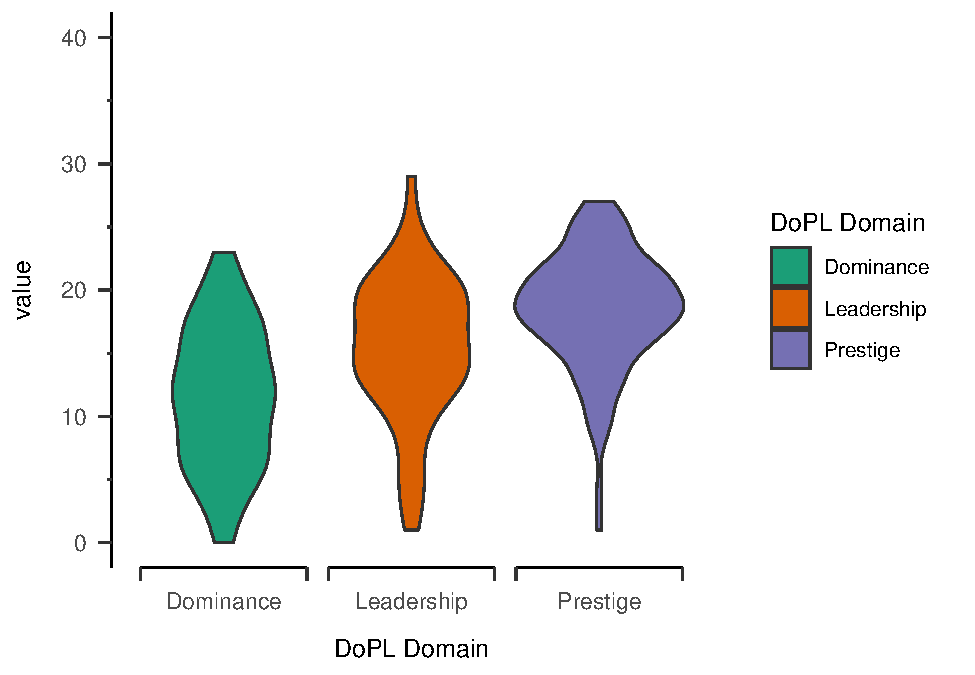
\includegraphics{DoPL-Experiment_files/figure-latex/unnamed-chunk-2-1.pdf}

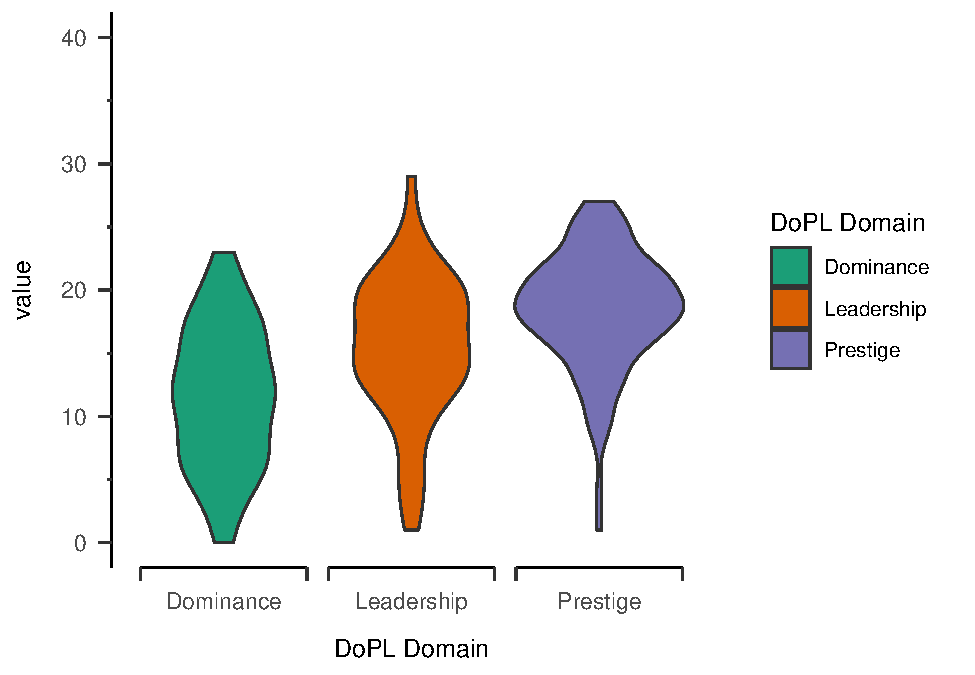
\includegraphics{DoPL-Experiment_files/figure-latex/unnamed-chunk-3-1.pdf}


\end{document}
